\documentclass{beamer}
\usepackage{color}
\usepackage{amsthm}
\usepackage{amssymb}
\usepackage{amsfonts}
\usepackage[T1]{fontenc}
\usepackage{lmodern}
\usepackage{comment}
\usepackage{tikz}
\usepackage{pgfpict2e}
\usepackage{verbatim}
\usepackage{textcomp}
\usepackage{amsmath}
\usepackage{listings}	
\usepackage{enumerate}
\usepackage[english]{babel}
\usepackage{times}
\usepackage{latexsym}    % to get LASY symbols
\usepackage{graphicx}    % to insert PostScript figures
\usepackage{cite}
\usepackage{rotating}    % for sideways tables/figures
\usepackage{xspace}
\usepackage{subfigure}
\usepackage{xmpmulti}
\usepackage[labelformat=empty]{caption}
\usepackage{algpseudocode}
\usepackage{tabularx}
\usepackage{fixltx2e}
\usepackage{algorithm}

\graphicspath{{figures/}}

\usetikzlibrary{matrix,arrows,decorations.pathmorphing}
\usetikzlibrary{positioning}
\newcommand{\myunit}{1 cm}
\newcommand{\hhlline}[3]{\draw (#1-#2-1.south west) -- (#1-#2-#3.south east);}
\newcommand{\toplline}[3]{\draw (#1-#2-1.north west) -- (#1-#2-#3.north east);}
\newcommand{\Ab}{\textbf{A}}
\newcommand{\Bb}{\textbf{B}}
\newcommand{\Cb}{\textbf{C}}
\newcommand{\tilep}{\texttt{tile}\xspace}
\newcommand{\inp}{\texttt{in}\xspace}
\newcommand{\dbp}{\texttt{db}\xspace}
\newcommand{\shapep}{\texttt{shape}\xspace}

\newcommand{\PADSEP}{0pt}

\newcommand{\constraints}{\ensuremath{\mathcal{T}}\xspace}
\newcommand{\format}[1]{\textit{#1}\xspace}
\newcommand{\generategroups}{\format{SuperblockAssignments}}
\newcommand{\extractgroups}{\format{extractGroups}}
\newcommand{\extracttables}{\format{extractTables}}
\newcommand{\learnconstraints}{\format{LearnConstraints}}
\newcommand{\findassignment}{\format{Subassignments}}
\newcommand{\postprocess}{\format{pruneRedundant}}
\newcommand{\constrainttorder}{\format{templateOrder}}
\newcommand{\template}{\format{constraint template}}
\newcommand{\sname}{\format{TaCLe}}


\newcommand{\CName}{Syntax\xspace}
\newcommand{\CSignature}{Signature\xspace}
\newcommand{\CFunction}{Definition\xspace}
\newcommand{\dependencies}{\ensuremath{\mathcal{D}}\xspace}
\newcommand{\groups}{\ensuremath{\mathcal{B}}\xspace}
\newcommand{\blocks}{\ensuremath{\mathcal{B}}\xspace}

\newcommand{\range}[3]{\ensuremath{#1[#2,#3]}}
\newcommand{\rangeto}[2]{#1{:}#2}
\newcommand{\rangeall}{:}

\newcommand{\eccalc}[2]{\ensuremath{#1 = #2}}
\newcommand{\ecrank}[2]{\eccalc{#1}{\textit{RANK}(#2)}}
\newcommand{\ecfkey}[2]{\ensuremath{\textit{FOREIGNKEY}(#1,#2)}}
\newcommand{\ecalldiff}[1]{\ensuremath{\textit{ALLDIFFERENT}(#1)}}
\newcommand{\eclookupf}[4]{\ensuremath{\textit{LOOKUP}_{\textit{#4}}(#1, #2, #3)}}
\newcommand{\eclookup}[4]{\eccalc{#1}{\eclookupf{#2}{#3}{#4}{}}}
\newcommand{\eclookupprod}[5]{\eccalc{#1}{#2 \times \eclookupf{#3}{#4}{#5}{}}}
\newcommand{\eclookupfuzzy}[4]{\eccalc{#1}{\eclookupf{#2}{#3}{#4}{fuzzy}}}
\newcommand{\ecperm}[1]{\ensuremath{\textit{PERMUTATION}(#1)}}
\newcommand{\ecseries}[1]{\ensuremath{\textit{SERIES}(#1)}}
\newcommand{\ecprod}[3]{\eccalc{#1}{#2 \times #3}}
\newcommand{\ecdiv}[3]{\eccalc{#1}{{#2} / {#3}}}
\newcommand{\ecdiff}[3]{\eccalc{#1}{#2 - #3}}
\newcommand{\ectotal}[3]{\eccalc{#1}{\textit{PREV}(#1) + #2 - #3}}
\newcommand{\ecproj}[2]{\eccalc{#1}{\textit{PROJECT}(#2)}}
\newcommand{\ecaggc}[3]{\eccalc{#2}{\textit{#1\textsubscript{col}}(#3)}}
\newcommand{\ecaggr}[3]{\eccalc{#2}{\textit{#1\textsubscript{row}}(#3)}}
\newcommand{\ecsumc}[2]{\eccalc{#1}{\textit{SUM\textsubscript{col}}(#2)}}
\newcommand{\ecsumr}[2]{\eccalc{#1}{\textit{SUM\textsubscript{row}}(#2)}}
\newcommand{\ecaggif}[5]{\eccalc{#2}{\textit{#1IF}(#3, #4, #5)}}
\newcommand{\ecsumif}[4]{\eccalc{#1}{\textit{SUMIF}(#2, #3, #4)}}
\newcommand{\ecsumprod}[3]{\eccalc{#1}{\textit{SUMPRODUCT}(#2, #3)}}

\newcommand{\numeric}{\format{numeric}}
\newcommand{\textual}{\format{textual}}
\newcommand{\integer}{\format{integer}}
\newcommand{\discrete}{\format{discrete}}
\newcommand{\plength}{\format{length}}
\newcommand{\psize}{\format{size}}
\newcommand{\ptype}{\format{type}}
\newcommand{\ptable}{\format{table}}
\newcommand{\por}{\format{orientation}}
\newcommand{\prows}{\format{rows}}
\newcommand{\pcols}{\format{columns}}
\newcommand{\nat}{\mathcal{N}}

\newcommand{\sg}{B}
\newcommand{\sbl}[1]{\ensuremath{B_{\textit{#1}}}}
\newcommand{\bsbl}[1]{\ensuremath{\mathbf{B_{\textit{#1}}}}}



\tikzset{
  node style sp/.style={draw,circle},
  node style ge/.style={circle},
  arrow style mul/.style={draw,sloped,midway,fill=white},
  arrow style plus/.style={midway,sloped,fill=white},
}

\definecolor{titleColor}{RGB}{0,179,0}
\definecolor{emphasizeColor}{RGB}{179,0,0}
\definecolor{otherColor}{RGB}{0,0,179}
\renewenvironment<>{example}[1][Example]{\begin{flushleft}\textcolor{otherColor}{#1}\\}{\end{flushleft}}
\usepackage{tikz}
\newcommand{\topline}{%
  \tikz[remember picture,overlay] {%
  \draw[black,solid] ([yshift=-30pt]current page.north west)
  -- ([yshift=-30pt,xshift=\paperwidth]current page.north west);
  }
}

\usetheme{boxes}
\usefonttheme{serif}
\usecolortheme{dove}
\beamertemplatenavigationsymbolsempty

\setbeamerfont{page number in head/foot}{size=\large}
\setbeamertemplate{footline}[frame number]

\setbeamertemplate{frametitle}
{
    \vspace{10pt}
    \insertframetitle
    \topline
}

\title{\sname}
\setbeamerfont{author}{shape=\itshape,family=\rmfamily}
\setbeamercolor{title}{fg=titleColor}
\setbeamercolor{frametitle}{fg=titleColor}
\setbeamercolor{frametitle}{fg=titleColor}
\setbeamercolor{example}{fg=otherColor}

\subtitle{Learning constraints in spreadsheets and tabular data}
%\author{Luc De Raedt, \underline{Sergey Paramonov}, Matthijs van Leeuwen}
\author{Sergey Paramonov, Samuel Kolb, Tias Guns, Luc De Raedt}
\institute{KU Leuven}
\date{\today}
\newtheorem{opr}{Definition}[section]

\newcommand{\ftmotivation}{Motivation}
\newcommand{\ftintro}{Formalization}
\newcommand{\ftapproach}{Approach}
\newcommand{\ftevaluation}{Evaluation}
\begin{document}

\begin{frame}
  \maketitle
\end{frame}

\begin{frame}[fragile]
\frametitle{\ftmotivation: Flash-fill}
%\transduration<0-15>{0}
    \multiinclude[<+->][format=png, graphics={width=\textwidth}]{frames/frame}
\end{frame}

\begin{frame}
  \frametitle{What is Flash-fill?}
\begin{itemize} \setlength{\itemsep}{+6mm}
    \item learns string transformation
    \item classic ML supervised setting
    \item one positive (or very few) example
    \item integrated into Excel
  \end{itemize}
  \vspace{10pt}


  {\Large \textbf{Key Question:} what if we make it unsupervised?}
\end{frame}

\begin{frame}[fragile]
  \frametitle{Can we recover formulas from a CSV file?}
  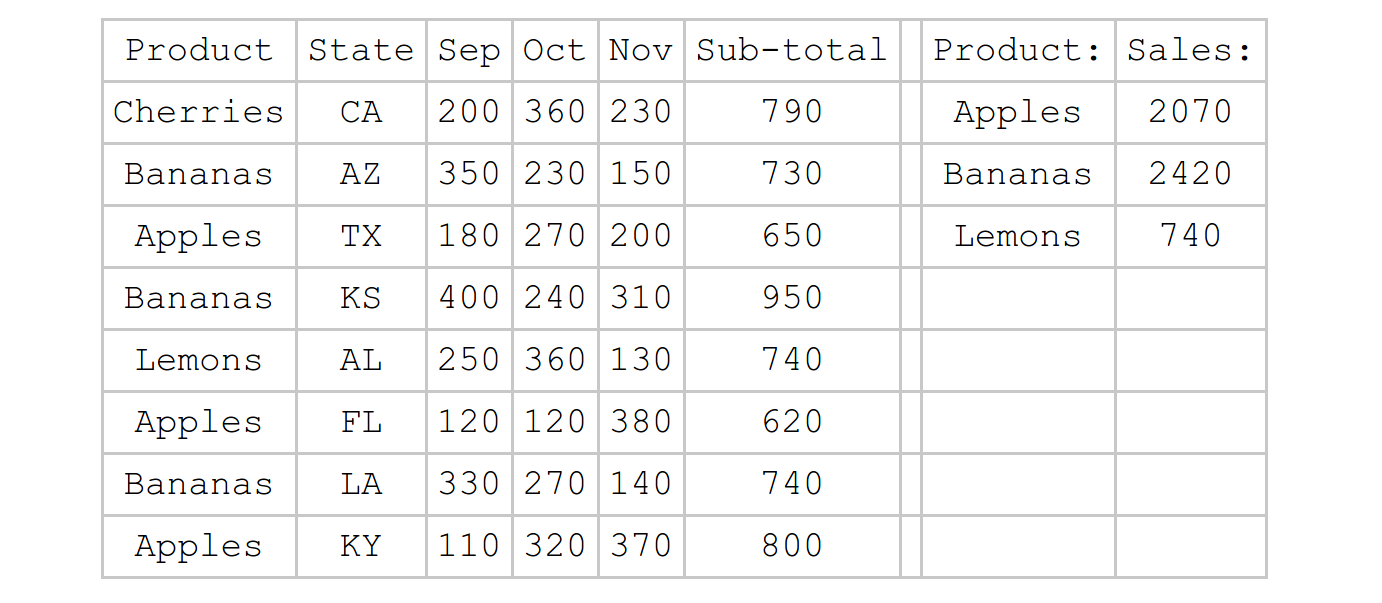
\includegraphics[width=\linewidth]{csv.png}

  \begin{itemize}[<+->]
    \item What are the formulas here?
    \item \begin{verbatim} T1[:, 6] = SUM(T1[:, 3:5], row) \end{verbatim}
  \item  \begin{verbatim} T2[:, 2] = SUMIF(T1[:, 1]=T2[:, 1], T1[:, 6]) \end{verbatim}
  \end{itemize}
\end{frame}

\begin{frame}
  \frametitle{What is new here?}
\begin{itemize} \setlength{\itemsep}{+6mm}
    \item Not typical data settings: no variables in columns and transactions in rows -- everything mixed
    \item Multi-relational learning (like sumif or lookup across multiple tables)
    \item Spreadsheet specific constraints -- fuzzy lookup or sumproduct
    \item Plenty of surprises: Nones, semi-structured data, numeric and textual
  \end{itemize}
\end{frame}


\begin{frame}
  \frametitle{Demo!}
  Demo comes here
\end{frame}








\begin{frame}[fragile]
  \frametitle{\ftintro}
  \begin{block}{Key Elements}
    \begin{itemize}
      \item<1-> Tables ($T$)
      \begin{itemize}
        \item $n \times m$ matrix
        \item Headerless
        \item Optional orientation
      \end{itemize}
      \item<2-> Blocks ($B$)
      \begin{itemize}
        \item Entire rows or entire columns (vectors)
        \item Fixed orientation
        \item Contiguous
        \item Type-consistent
      \end{itemize}
    \end{itemize}
  \end{block}
\end{frame}


\begin{frame}[fragile]
  \frametitle{\ftintro}
  \begin{block}{Example}
    \begin{figure}
      \centering
      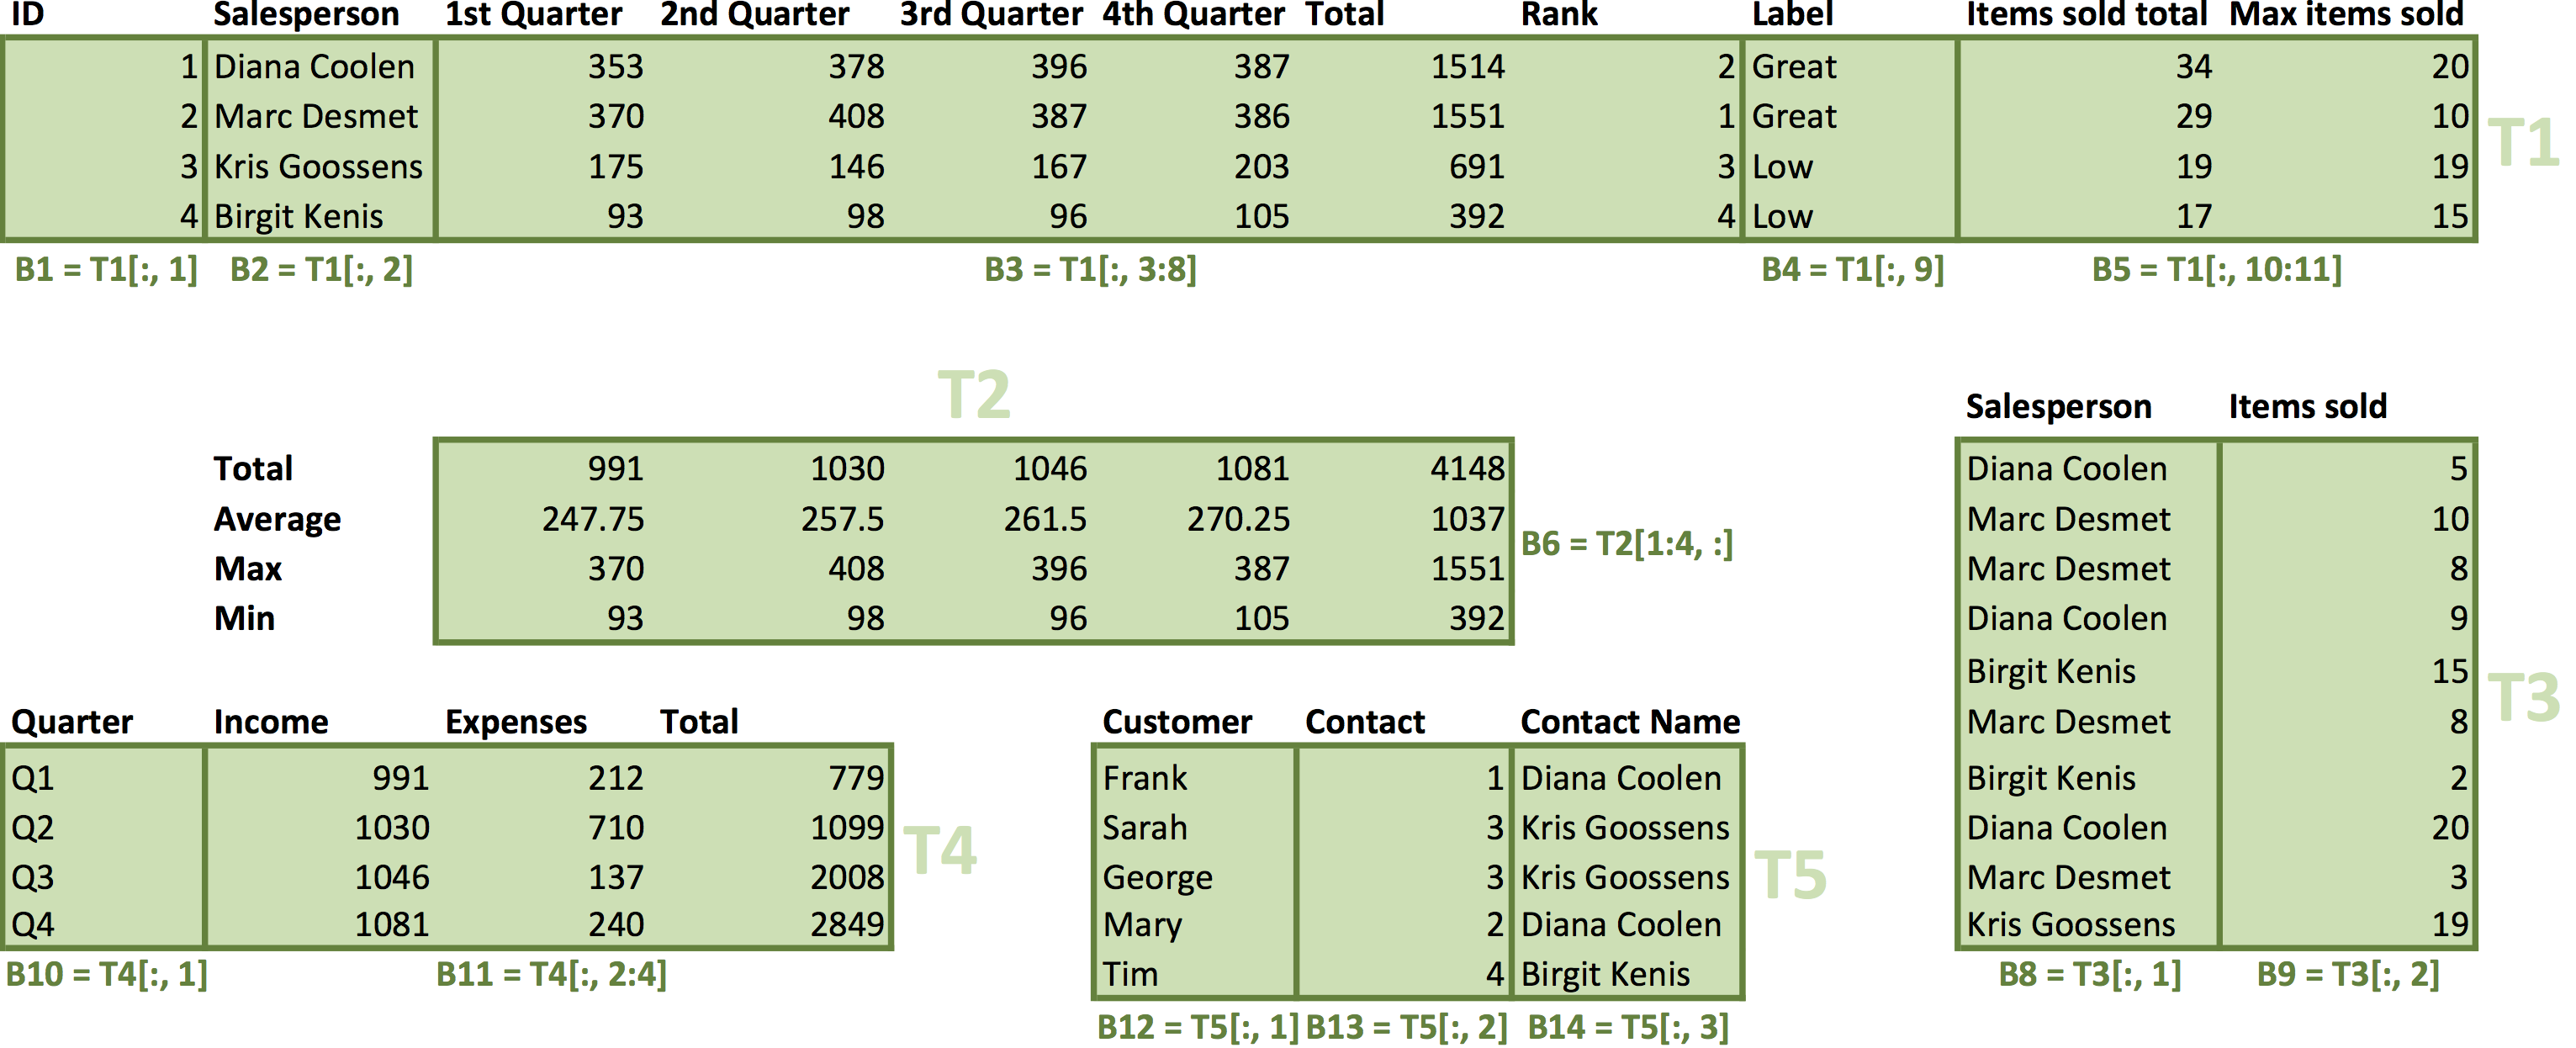
\includegraphics[width=1\textwidth]{Demo2.png}
    \end{figure}
  \end{block}
\end{frame}


\begin{frame}[fragile]
  \frametitle{\ftintro}
  \begin{block}{Block containment}
  \begin{itemize}
    \item $B' \sqsubseteq B$
    \begin{itemize}
      \item $B'$ subblock of $B$
      \item $B$ superblock of $B'$
    \end{itemize}
  \end{itemize}
  \end{block}
\end{frame}


\begin{frame}[fragile]
  \frametitle{\ftintro}
  \begin{block}{Example}
    \begin{figure}
      \centering
      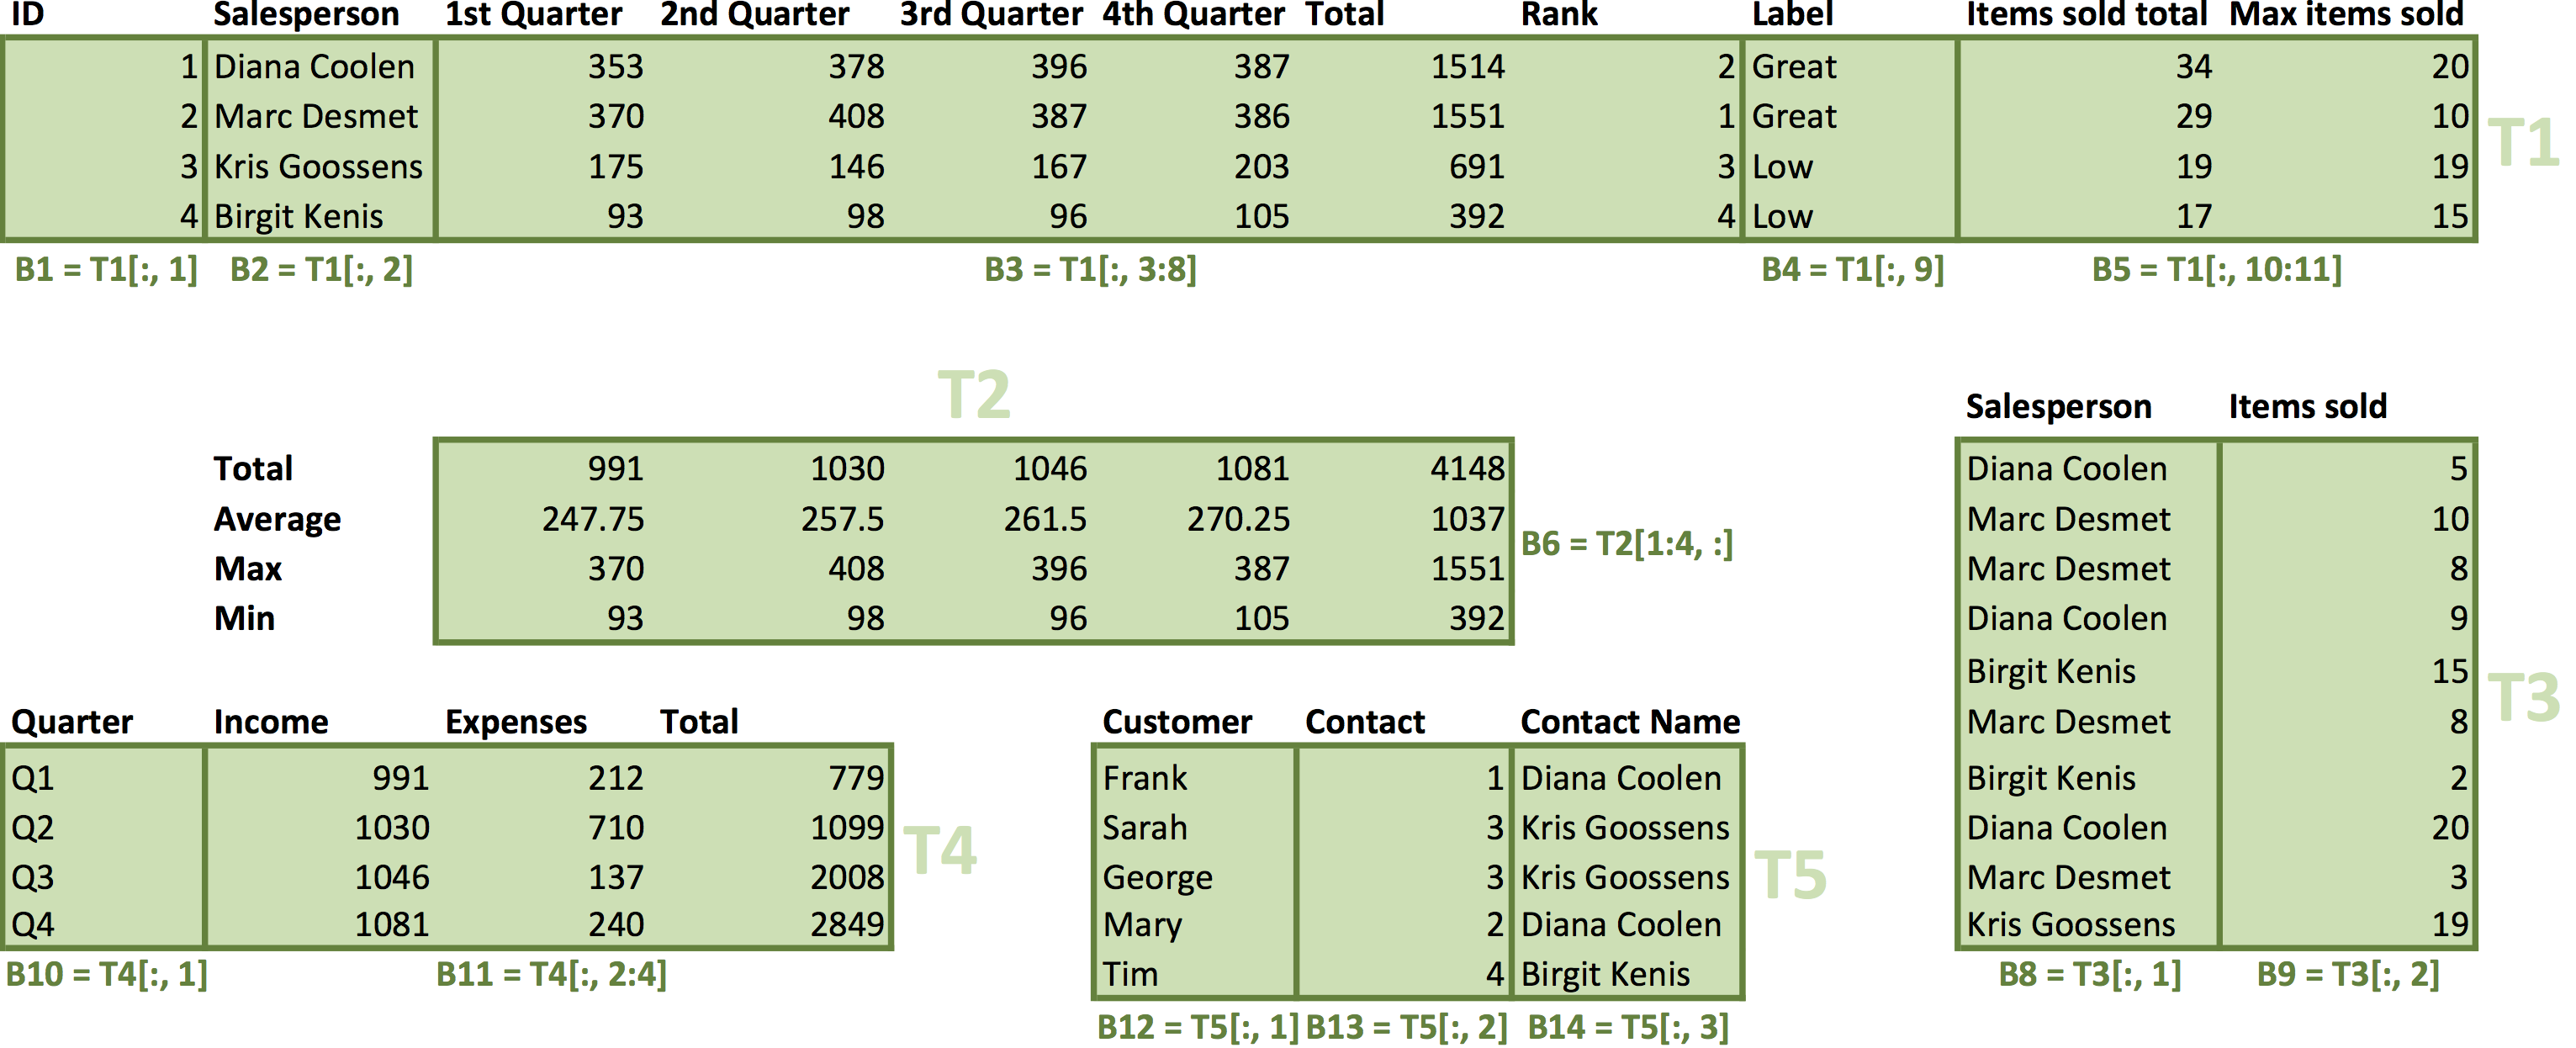
\includegraphics[width=1\textwidth]{Demo2.png}
    \end{figure}
  \end{block}
\end{frame}


\newcommand{\sigc}{\ensuremath{\format{Sig}_s}}
\newcommand{\defc}{\ensuremath{\format{Def}_s}}


\begin{frame}[fragile]
  \frametitle{\ftintro}
  \begin{block}{Constraint templates}
    \begin{itemize}
      \item Syntax
      \begin{itemize}
        \item Syntactic form, e.g. $\ecalldiff{\sg_x}$
        \item In logic: relation / predicate
      \end{itemize}
      \item Signature
        \begin{itemize}
          \item Requirements on arguments, e.g. $\discrete(\sg_x)$
          \item In logic: bias ($\sigc$)
        \end{itemize}
      \item Definition
        \begin{itemize}
          \item Actual definition, e.g. $i \neq j$: $\sg_x[i] \neq \sg_x[j]$
          \item In logic: ackground knowledge ($\defc$)
        \end{itemize}
    \end{itemize}
  \end{block}
\end{frame}


\begin{frame}[fragile]
  \frametitle{\ftintro}
  \begin{block}{Lookup}<1->
    \begin{itemize}
      \item Syntax: \eclookup{\sbl{r}}{\sbl{fk}}{\sbl{pk}}{\sbl{val}}
      \item Signature: $\sbl{fk}$ and $\sbl{pk}$ are $\discrete$; arguments $\{\sbl{fk}, \sbl{r}\}$ and $\{\sbl{pk}, \sbl{val}\}$ within the same set have the same \plength, \ptable and \por; $\sbl{r}$ and~$\sbl{val}$ have the same type; and \ecfkey{\sbl{fk}}{\sbl{pk}}.
      \item Definition: $\sbl{r}[i] = \sbl{val}[j]$ where $\sbl{pk}[j] = \sbl{fk}[i]$
    \end{itemize}
  \end{block}
  \begin{block}{Row-wise sum}<2->
    \begin{itemize}
      \item Syntax: $\ecsumr{\sg_r}{\mathbf{\sg_x}}$
      \item Signature: $\sg_r$ and $\mathbf{\sg_x}$ are $\numeric$; $\pcols(\mathbf{\sg_x}) \geq 2$; and $\prows(\mathbf{\sg_x}) = \plength(\sg_r)$
      \item Definition: $B_r[i] = \sum_{j = 1}^{\pcols(\bsbl{x})} \mathit{row}(i, \bsbl{x})[j]$
    \end{itemize}
  \end{block}
\end{frame}


\newcommand{\temps}{\ensuremath{S}}

\begin{frame}[fragile]
\frametitle{\ftapproach}
\begin{block}{High level algorithm}
  \begin{algorithm}[H]
  \begin{algorithmic}[1]
    \footnotesize
    \State \textbf{Input:} $\temps$ -- constraint templates, $\blocks$ -- maximal blocks
    \State \textbf{Output:} $C$ -- learned constraints

    \Procedure{LearnConstraints}{$\blocks$, $\temps$}
      \State $C \gets \emptyset$ %\Comment{The set of constraints}
      \ForAll{$s~\mathbf{in}~\temps$} \label{algo:tcl:for}
        %\State $n \gets$ number of arguments of template $s$
        \State $A \gets \generategroups(s, \blocks)$  \label{algo:tcl:super}
        \ForAll{$(B_1, \dots, B_n) \in A$}
        \State{$A' \gets \findassignment(s, (B_1,\dots,B_n))$}
        \ForAll{$(B_1',\dots,B_n') \in A'$}
            \State $C \gets C \cup \{ c_s(B_1', \dots, B_n') \}$
          \EndFor
        \EndFor
      \EndFor
      \State \Return $C$
    \EndProcedure
\end{algorithmic}
\end{algorithm}
\end{block}
\end{frame}

\begin{frame}[fragile]
\frametitle{\ftapproach}
\begin{block}{Intuition}
  \begin{itemize}
    \setlength{\itemsep}{+5mm}
    \item Example: $\ecsumc{Y}{X}$
    \item Step 1: Find superblock assignments (i.e. suitable blocks)
    \begin{itemize}
      \item Assignments \textit{compatible} signature, relax where necessary
      \item e.g. $\numeric(X)$, $\numeric(Y)$, $\pcols(X) \geq 2$
      \item e.g. $\prows(X) = \plength(Y)$
    \end{itemize}
    \item Step 2: Find all constraints over subblocks of the superblock assignments
    \begin{itemize}
      \item Find \textit{subassignments} that satisfy the signature and the definition
      \item e.g. find subblocks for $X$ and $Y$ such that $Y[i] = \sum \mathit{column~i}$
    \end{itemize}
  \end{itemize}
\end{block}

\end{frame}

\begin{frame}[fragile]
  \frametitle{\ftapproach}
  \begin{block}{Illustration}
    \begin{figure}
      \centering
      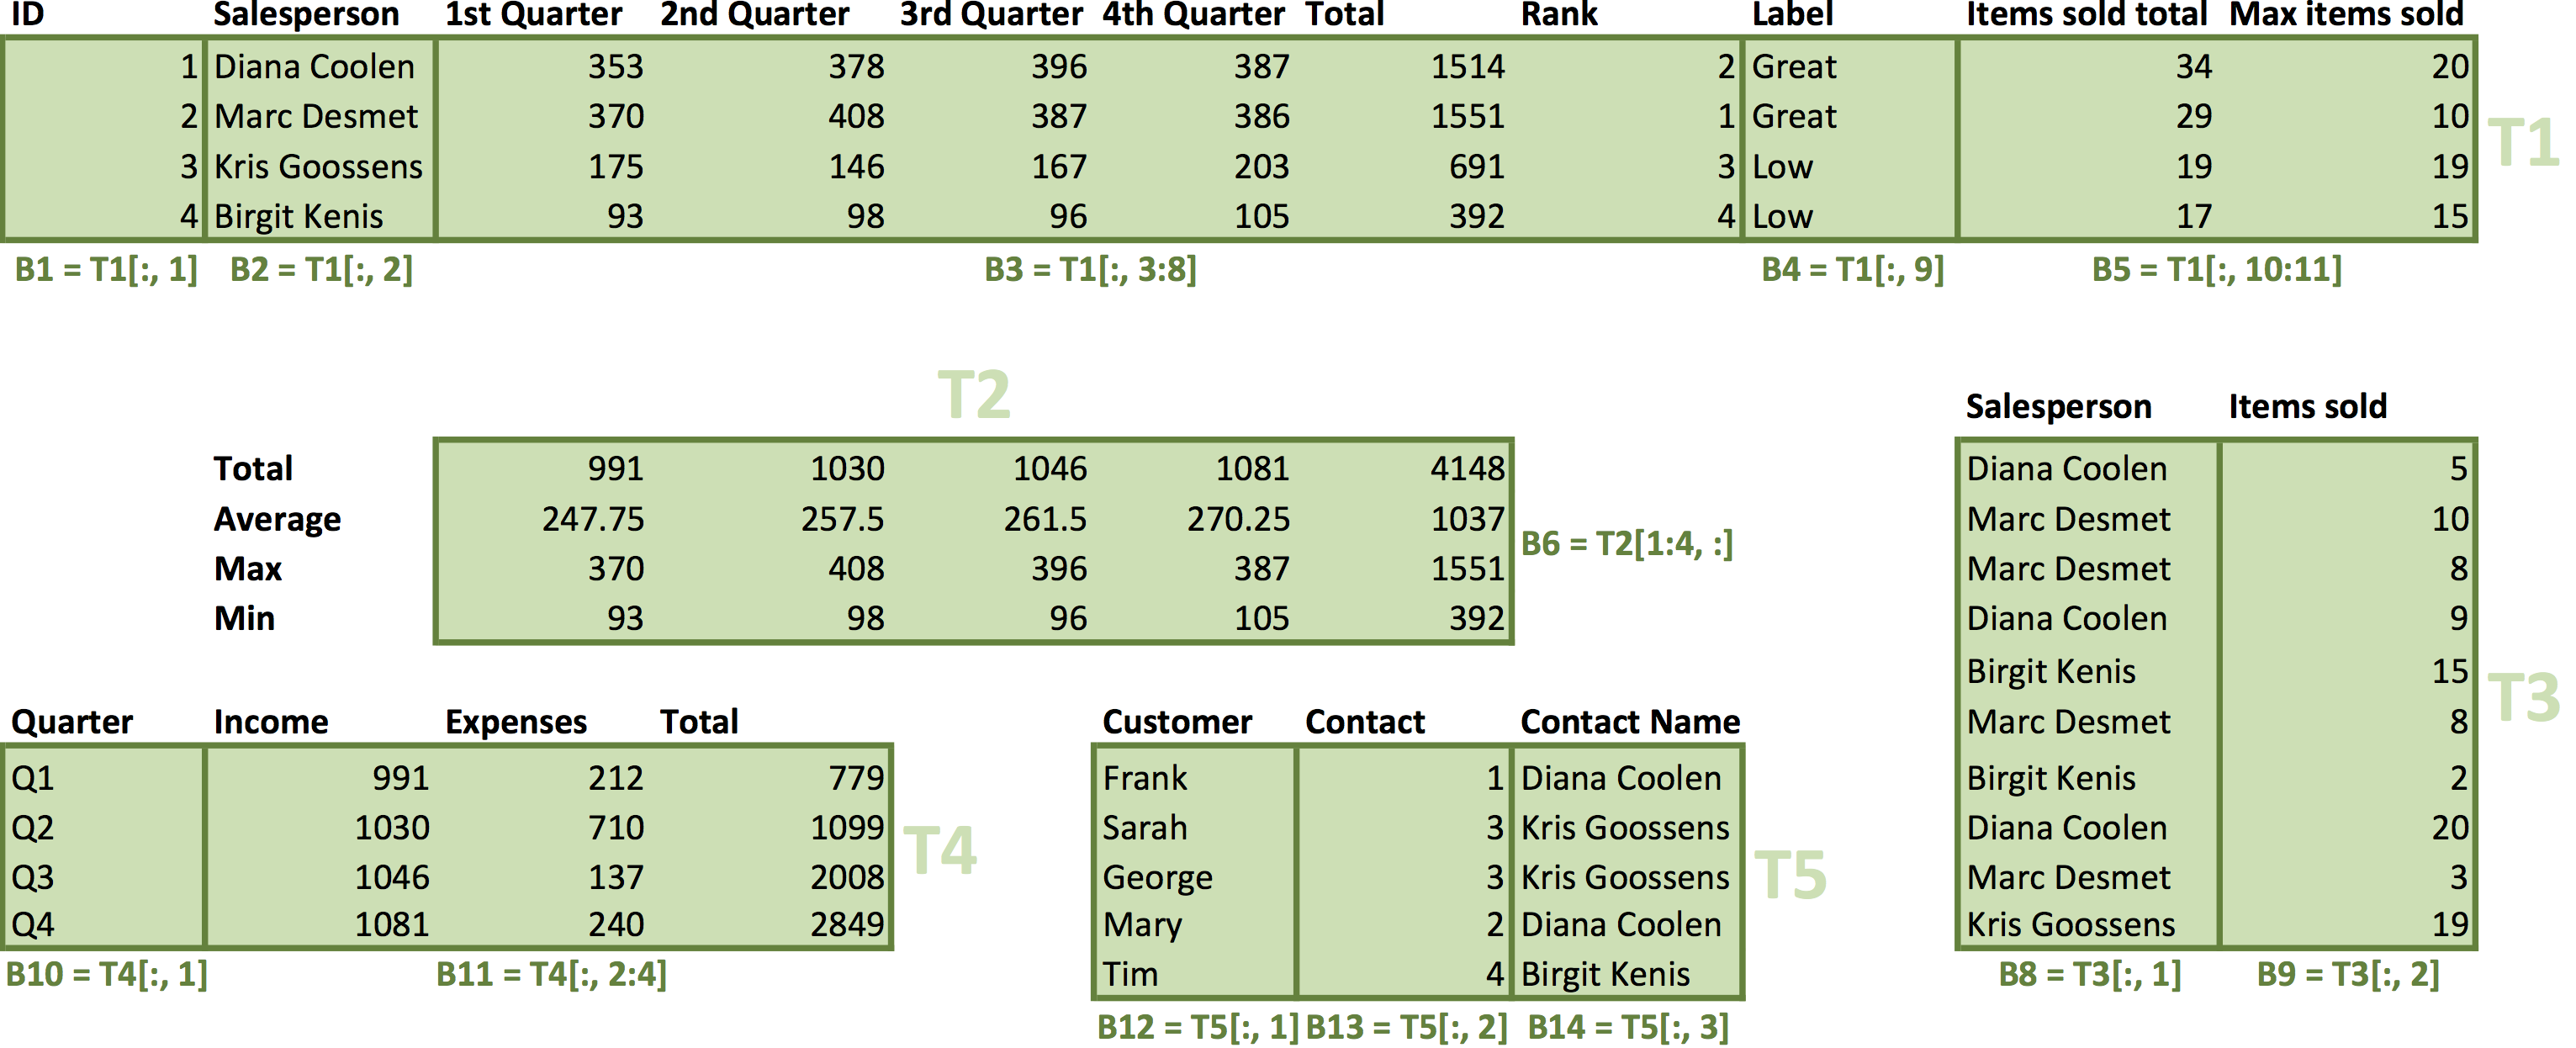
\includegraphics[width=1\textwidth]{Demo2.png}
    \end{figure}
  \end{block}
\end{frame}


\begin{frame}[fragile]
  \frametitle{\ftapproach}
  \begin{block}{Dependencies}
    \begin{figure}
      \centering
      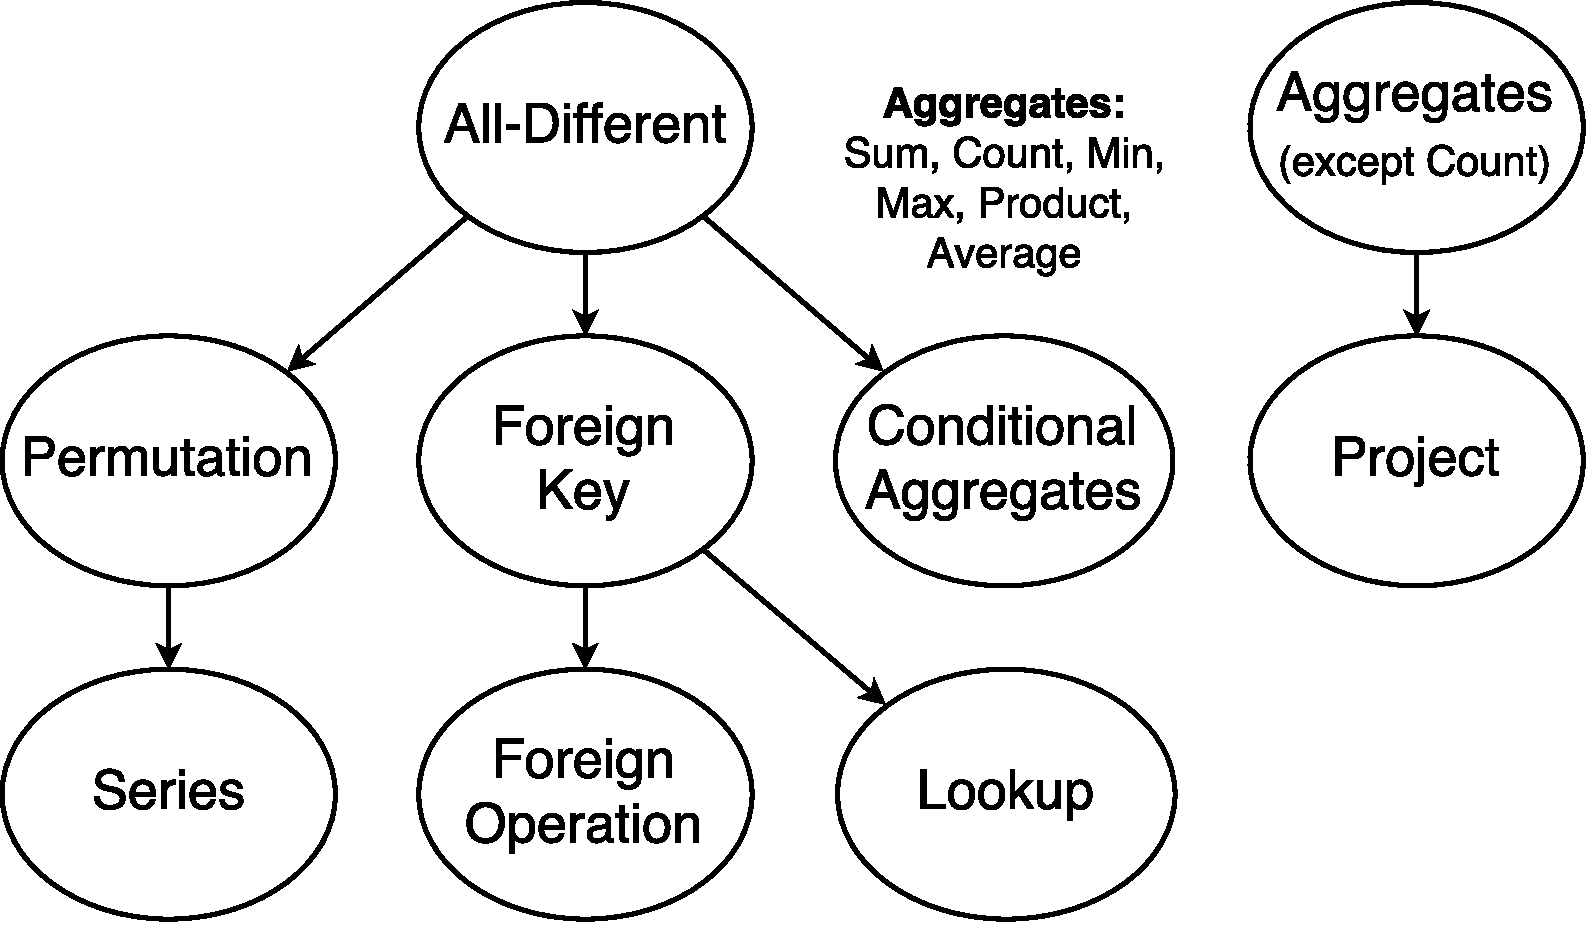
\includegraphics[width=0.7\textwidth]{dependencies.pdf}
    \end{figure}
  \end{block}
\end{frame}


\begin{frame}[fragile]
\frametitle{\ftevaluation}
\begin{block}{Evaluation questions}
  \begin{itemize}
    \item Recall (\textit{Q1})
    \item Precision (\textit{Q2})
    \item Speed (\textit{Q3})
  \end{itemize}
\end{block}
\pause
\begin{block}{Structure}
  \begin{itemize}
    \item Method
    \item Case study
    \item Benchmark
    \item Testing the limits
  \end{itemize}
\end{block}
\end{frame}


\begin{frame}[fragile]
\frametitle{\ftevaluation}
\begin{block}{Method}
  \begin{itemize}
    \item<1-> Benchmark spreadsheets collected
    \begin{itemize}
      \item Exercise session
      \item Online tutorials
      \item \textit{Data} spreadsheets (e.g. crime statistics, fincancial data)
    \end{itemize}
    \item<2-> Convert all spreadsheets to CSV files
    \item<3-> Manually specify ground-truth: \textit{intended} constraints
    \begin{itemize}
      \item Based on original formulas, context, headers (intuition)
      \item Structural constraints are ignored
    \end{itemize}
  \end{itemize}
\end{block}
\end{frame}


\begin{frame}[fragile]
  \frametitle{\ftevaluation}
  \begin{block}{Case study}
    \begin{figure}
      \centering
      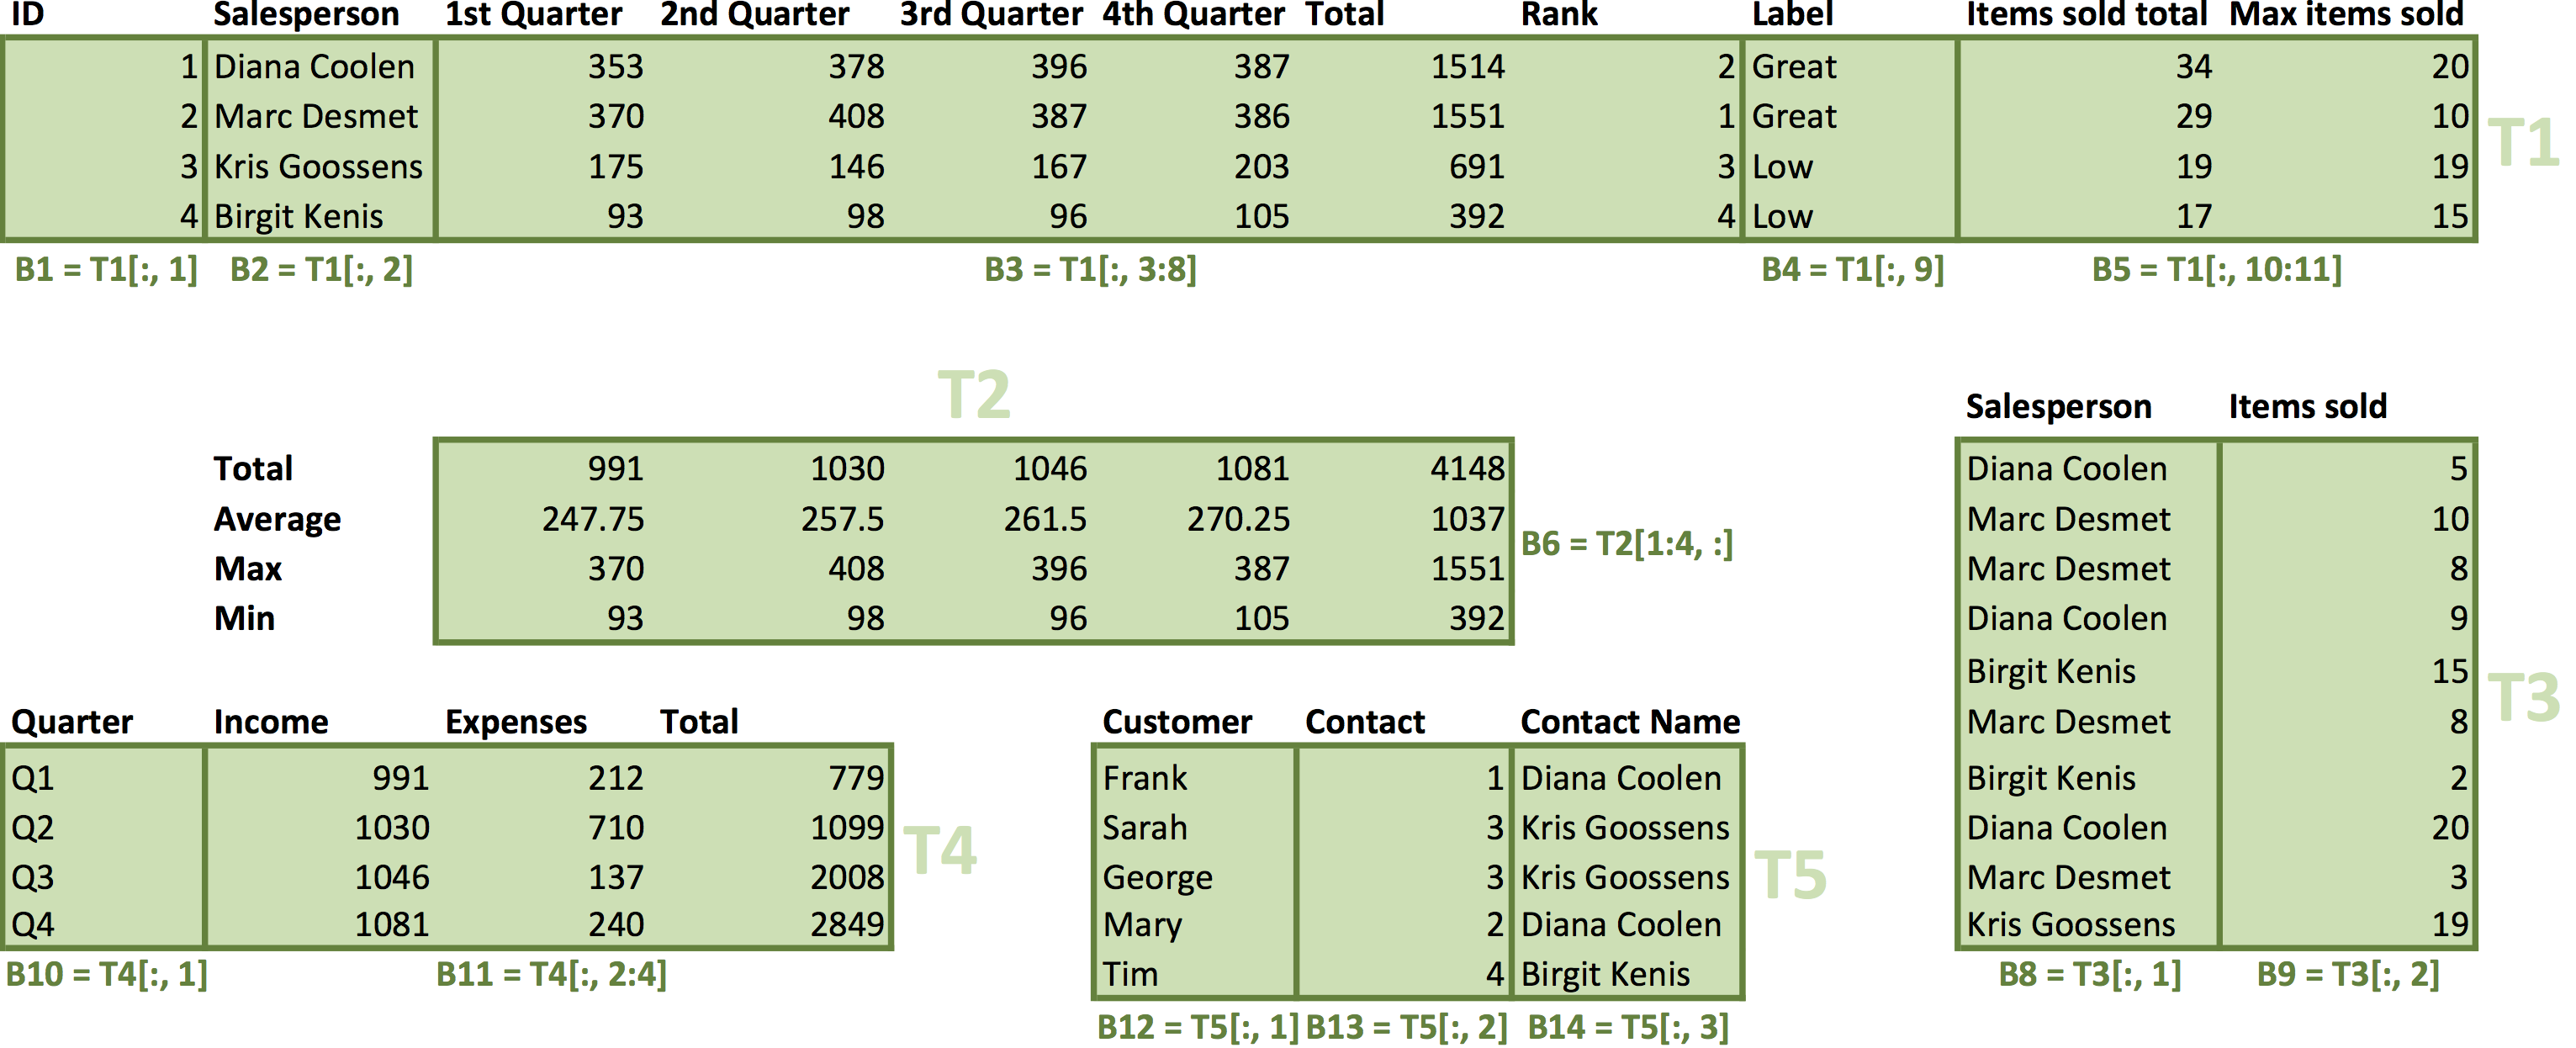
\includegraphics[width=1\textwidth]{Demo2.png}
    \end{figure}
  \end{block}
\end{frame}


\begin{frame}[fragile]
\frametitle{\ftevaluation}
  \begin{block}{Case study}
    {\tiny
      \begin{align*}
        % Table 1
        &~\ecseries{\range{T_{1}}{\rangeall}{1}} \\
  %
  %      &~\ecperm{\range{T_{1}}{\rangeall}{1}}, \ecperm{\range{T_{1}}{\rangeall}{8}} \\
  %
        &~\ecrank{\range{T_{1}}{\rangeall}{1}}{\range{T_{1}}{\rangeall}{5}}^*\\
        &~\ecrank{\range{T_{1}}{\rangeall}{1}}{\range{T_{1}}{\rangeall}{6}}^* \\
        &~\ecrank{\range{T_{1}}{\rangeall}{1}}{\range{T_{1}}{\rangeall}{10}}^*\\
        &~\ecrank{\range{T_{1}}{\rangeall}{8}}{\range{T_{1}}{\rangeall}{7}} \\
        &~\ecrank{\range{T_{1}}{\rangeall}{8}}{\range{T_{1}}{\rangeall}{3}}^*\\
        &~\ecrank{\range{T_{1}}{\rangeall}{8}}{\range{T_{1}}{\rangeall}{4}}^* \\
  %
        &~\ecsumr{\range{T_{1}}{\rangeall}{7}}{\range{T_{1}}{\rangeall}{\rangeto{3}{6}}} \\
  %
        &~\ecaggif{\textit{SUM}}{\range{T_{1}}{\rangeall}{10}}{\range{T_{3}}{\rangeall}{1}}{\range{T_{1}}{\rangeall}{2}}{\range{T_{3}}{\rangeall}{2}} \\
  %
        &~\ecaggif{\textit{MAX}}{\range{T_{1}}{\rangeall}{11}}{\range{T_{3}}{\rangeall}{1}}{\range{T_{1}}{\rangeall}{2}}{\range{T_{3}}{\rangeall}{2}} \\
  %
      % Table 2
        &~\ecsumc{\range{T_{2}}{1}{\rangeall}}{\range{T_{1}}{\rangeall}{\rangeto{3}{7}}} \\
  %
        &~\ecaggc{\textit{AVERAGE}}{\range{T_{2}}{2}{\rangeall}}{\range{T_{1}}{\rangeall}{\rangeto{3}{7}}} \\
  %
        &~\ecaggc{\textit{MAX}}{\range{T_{2}}{3}{\rangeall}}{\range{T_{1}}{\rangeall}{\rangeto{3}{7}}},  \\
  %
        &~\ecaggc{\textit{MIN}}{\range{T_{2}}{4}{\rangeall}}{\range{T_{1}}{\rangeall}{\rangeto{3}{7}}} \\
  %
      % Table 4
        &~\ecsumc{\range{T_{4}}{\rangeall}{2}}{\range{T_{1}}{\rangeall}{\rangeto{3}{6}}} \\
  %
        &~\range{T_{4}}{\rangeall}{4} = PREV(\range{T_{4}}{\rangeall}{4}) + \range{T_{4}}{\rangeall}{2} - \range{T_{4}}{\rangeall}{3} \\
  %
      % Table 5
        &~\eclookup{\range{T_{5}}{\rangeall}{2}}{\range{T_{5}}{\rangeall}{3}}{\range{T_{1}}{\rangeall}{2}}{\range{T_{1}}{\rangeall}{1}}^* \\
  %
        &~\eclookup{\range{T_{5}}{\rangeall}{3}}{\range{T_{5}}{\rangeall}{2}}{\range{T_{1}}{\rangeall}{1}}{\range{T_{1}}{\rangeall}{2}}
      \end{align*}}

  \end{block}
\end{frame}


\begin{frame}[fragile]
  \frametitle{\ftevaluation}
  \begin{block}{Case study}
    \begin{itemize}
      \item<1-> Recall intended constraints: $1.0$
      \item<2-> Precision: $\frac{12}{18} = 0.67$
      \begin{itemize}
        \item Not that high
      \end{itemize}
      \item<3-> Few seconds
    \end{itemize}
  \end{block}
\end{frame}


\begin{frame}[fragile]
\frametitle{\ftevaluation}
\begin{block}{Benchmark}
  {\small\setlength{\tabcolsep}{0.33em}
    \begin{table}[]
      \centering
      \label{tbl:category_overview}
      \begin{tabularx}{\linewidth}{lccccccc}
        & \multicolumn{2}{c}{\textbf{Exercises} (9)} & \multicolumn{2}{c}{\textbf{Tutorials} (21)} & \multicolumn{2}{c}{\textbf{Data} (4)} \\
        & Overall & Sheet avg & Overall & Sheet avg & Overall & Sheet avg \\ \hline
        \textbf{Tables} & 19 & 2.11 & 48 & 2.29 & 4 & 1 \\ \hline
        \textbf{Cells} & 1231 & 137 & 1889 & 90 & 2320 & 580 \\ \hline
        \textbf{\begin{tabular}[c]{@{}l@{}}Intended\\[-4pt] Constraints\end{tabular}} & 34 & 3.78 & 52 & 2.48 & 6 & 1.50
      \end{tabularx}
    \end{table}
  }
  \end{block}
\end{frame}


\begin{frame}[fragile]
\frametitle{\ftevaluation}
  \begin{block}{Benchmark}
    {\small\setlength{\tabcolsep}{0.33em}
      \begin{table}[]
        \centering
        \label{tbl:category_overview}
        \begin{tabularx}{\linewidth}{lccccccc}
          & \multicolumn{2}{c}{\textbf{Exercises} (9)} & \multicolumn{2}{c}{\textbf{Tutorials} (21)} & \multicolumn{2}{c}{\textbf{Data} (4)} \\
          & Overall & Sheet avg & Overall & Sheet avg & Overall & Sheet avg \\ \hline
          \textbf{Recall} & 0.85 & 0.83 & 0.88 & 0.87 & 1.00 & 1.00 \\ \hline
          \textbf{\begin{tabular}[c]{@{}l@{}}Recall\\[-4pt] Supported\end{tabular}} & 1.00 & 1.00 & 1.00 & 1.00 & 1.00 & 1.00 \\ \hline
          \textbf{Precision} & 0.97 & 0.98 & 0.70 & 0.91 & 1.00 & 1.00 \\ \hline
          \textbf{Speed (s)} & 1.62 & 0.18 & 1.76 & 0.08 & 0.81 & 0.20
        \end{tabularx}
      \end{table}
    }
    \pause
    \begin{itemize}
      \item<+-> Q1. How many intended constraints are found by \sname?
      \begin{itemize}
        \item High recall
        \item All supported constraints always found  \end{itemize}
      \item<+-> Q2. How precise is \sname?
      \begin{itemize}
        \item Precise on most spreadsheets
        \item Duplicates / multiple ways to calculate thwart precision
      \end{itemize}
      \item<+-> Q3. How fast is \sname?
      \begin{itemize}
        \item Dependencies crucial
      \end{itemize}
    \end{itemize}
  \end{block}
\end{frame}


\begin{frame}[fragile]
\frametitle{\ftevaluation}
\begin{block}{Benchmark}
  \begin{figure}[t]
    \centering
    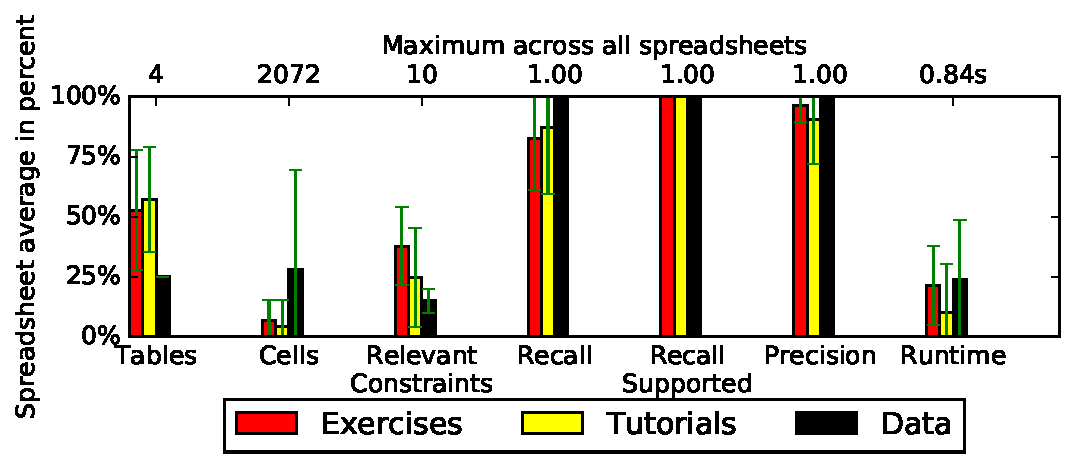
\includegraphics[width=1\linewidth]{comparison.pdf}
  \end{figure}
\end{block}
\end{frame}


\begin{frame}[fragile]
  \frametitle{\ftevaluation}
  \begin{block}{Testing the limits}
    \begin{itemize}
      \item<1-> ``exps\_tias''
      \begin{itemize}
        \item 6 tables
        \item 531 cells
        \item Many duplicate columns across tables
      \end{itemize}
      \item<2-> Q1 Recall: $1.0$
      \item<3-> Q2 Precision: $0.52 / 0.11$ (with / without equalities)
      \begin{itemize}
        \item Post-processing step (entailment / heuristic)
      \end{itemize}
      \item<4-> Q3 Speed: $14.30s$
    \end{itemize}
  \end{block}
\end{frame}

\begin{frame}[fragile]
  \frametitle{Applications}
  \begin{block}{Autocompletion}
    \begin{figure}
      \begin{center}
        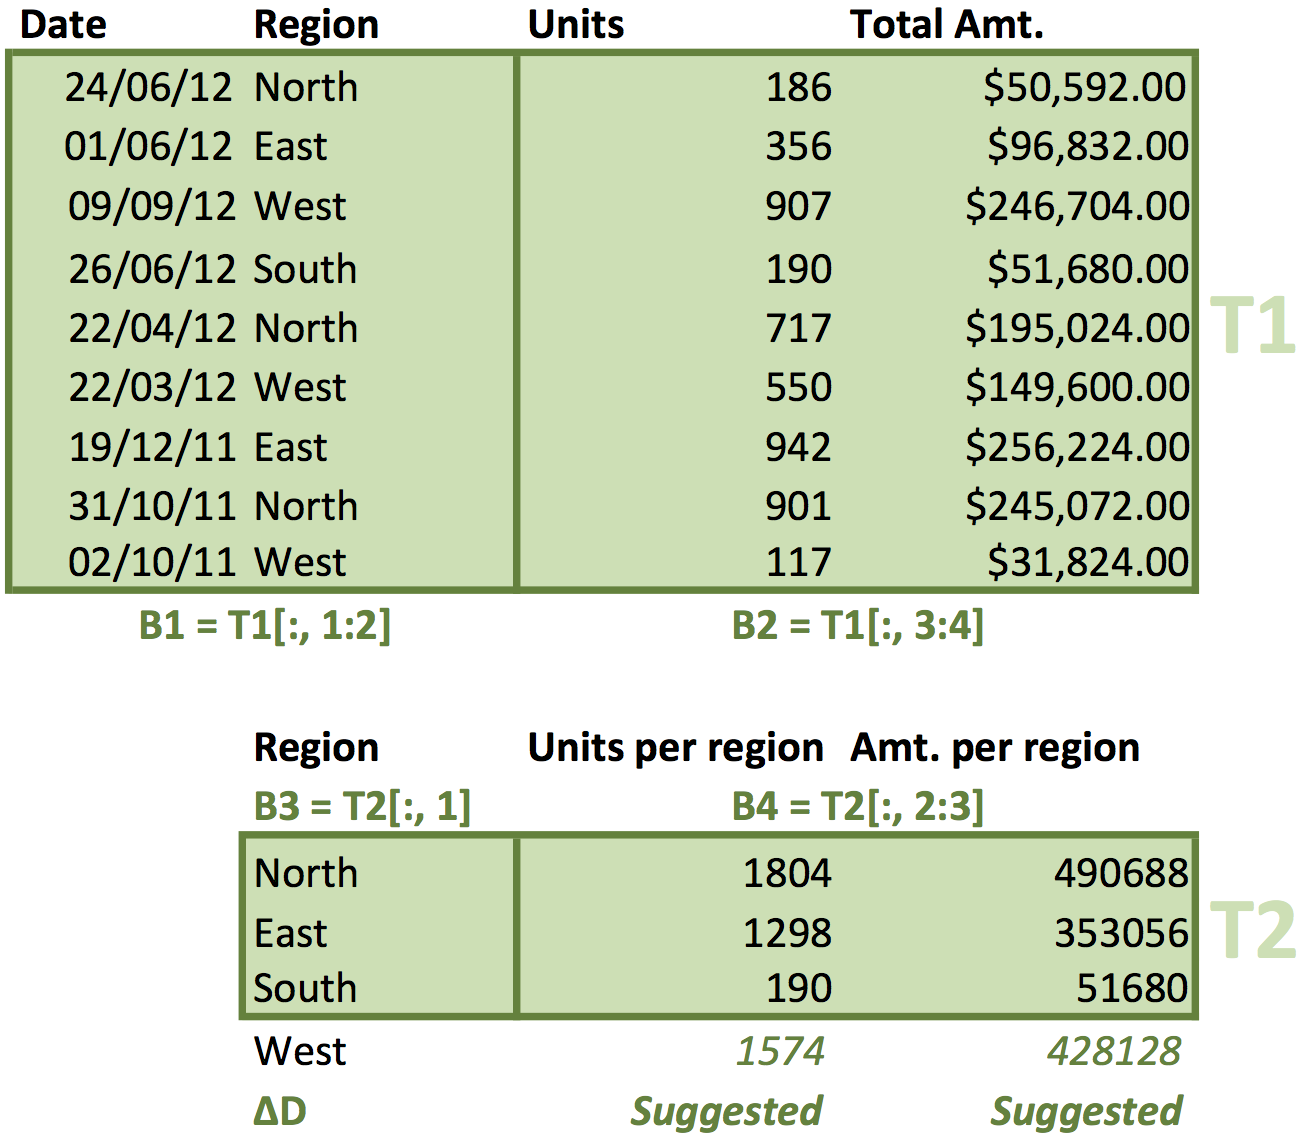
\includegraphics[width=0.65\linewidth]{learning.png}
      \end{center}
    \end{figure}
  \end{block}
\end{frame}


\begin{frame}[fragile]
  \frametitle{Conclusion}
  \begin{block}{Conclusion}
    \begin{itemize}
      \item<+-> Approach that learns constraints in spreadsheet
      \begin{itemize}
        \item<+-> Accurate
        \item<+-> Rather precise
        \item<+-> Efficient
      \end{itemize}
    \end{itemize}
  \end{block}
  \pause
  \begin{block}{Future work}
    \begin{itemize}
      \item<+-> Nested constraints
      \item<+-> Sub vector-size
      \item<+-> Post-processing (heuristic / entailment)
      \item<+-> Noise
    \end{itemize}
  \end{block}
\end{frame}


\begin{frame}[fragile]
  \frametitle{Conclusion}
  \begin{block}{Questions?}
    \begin{figure}[t]
      \centering
      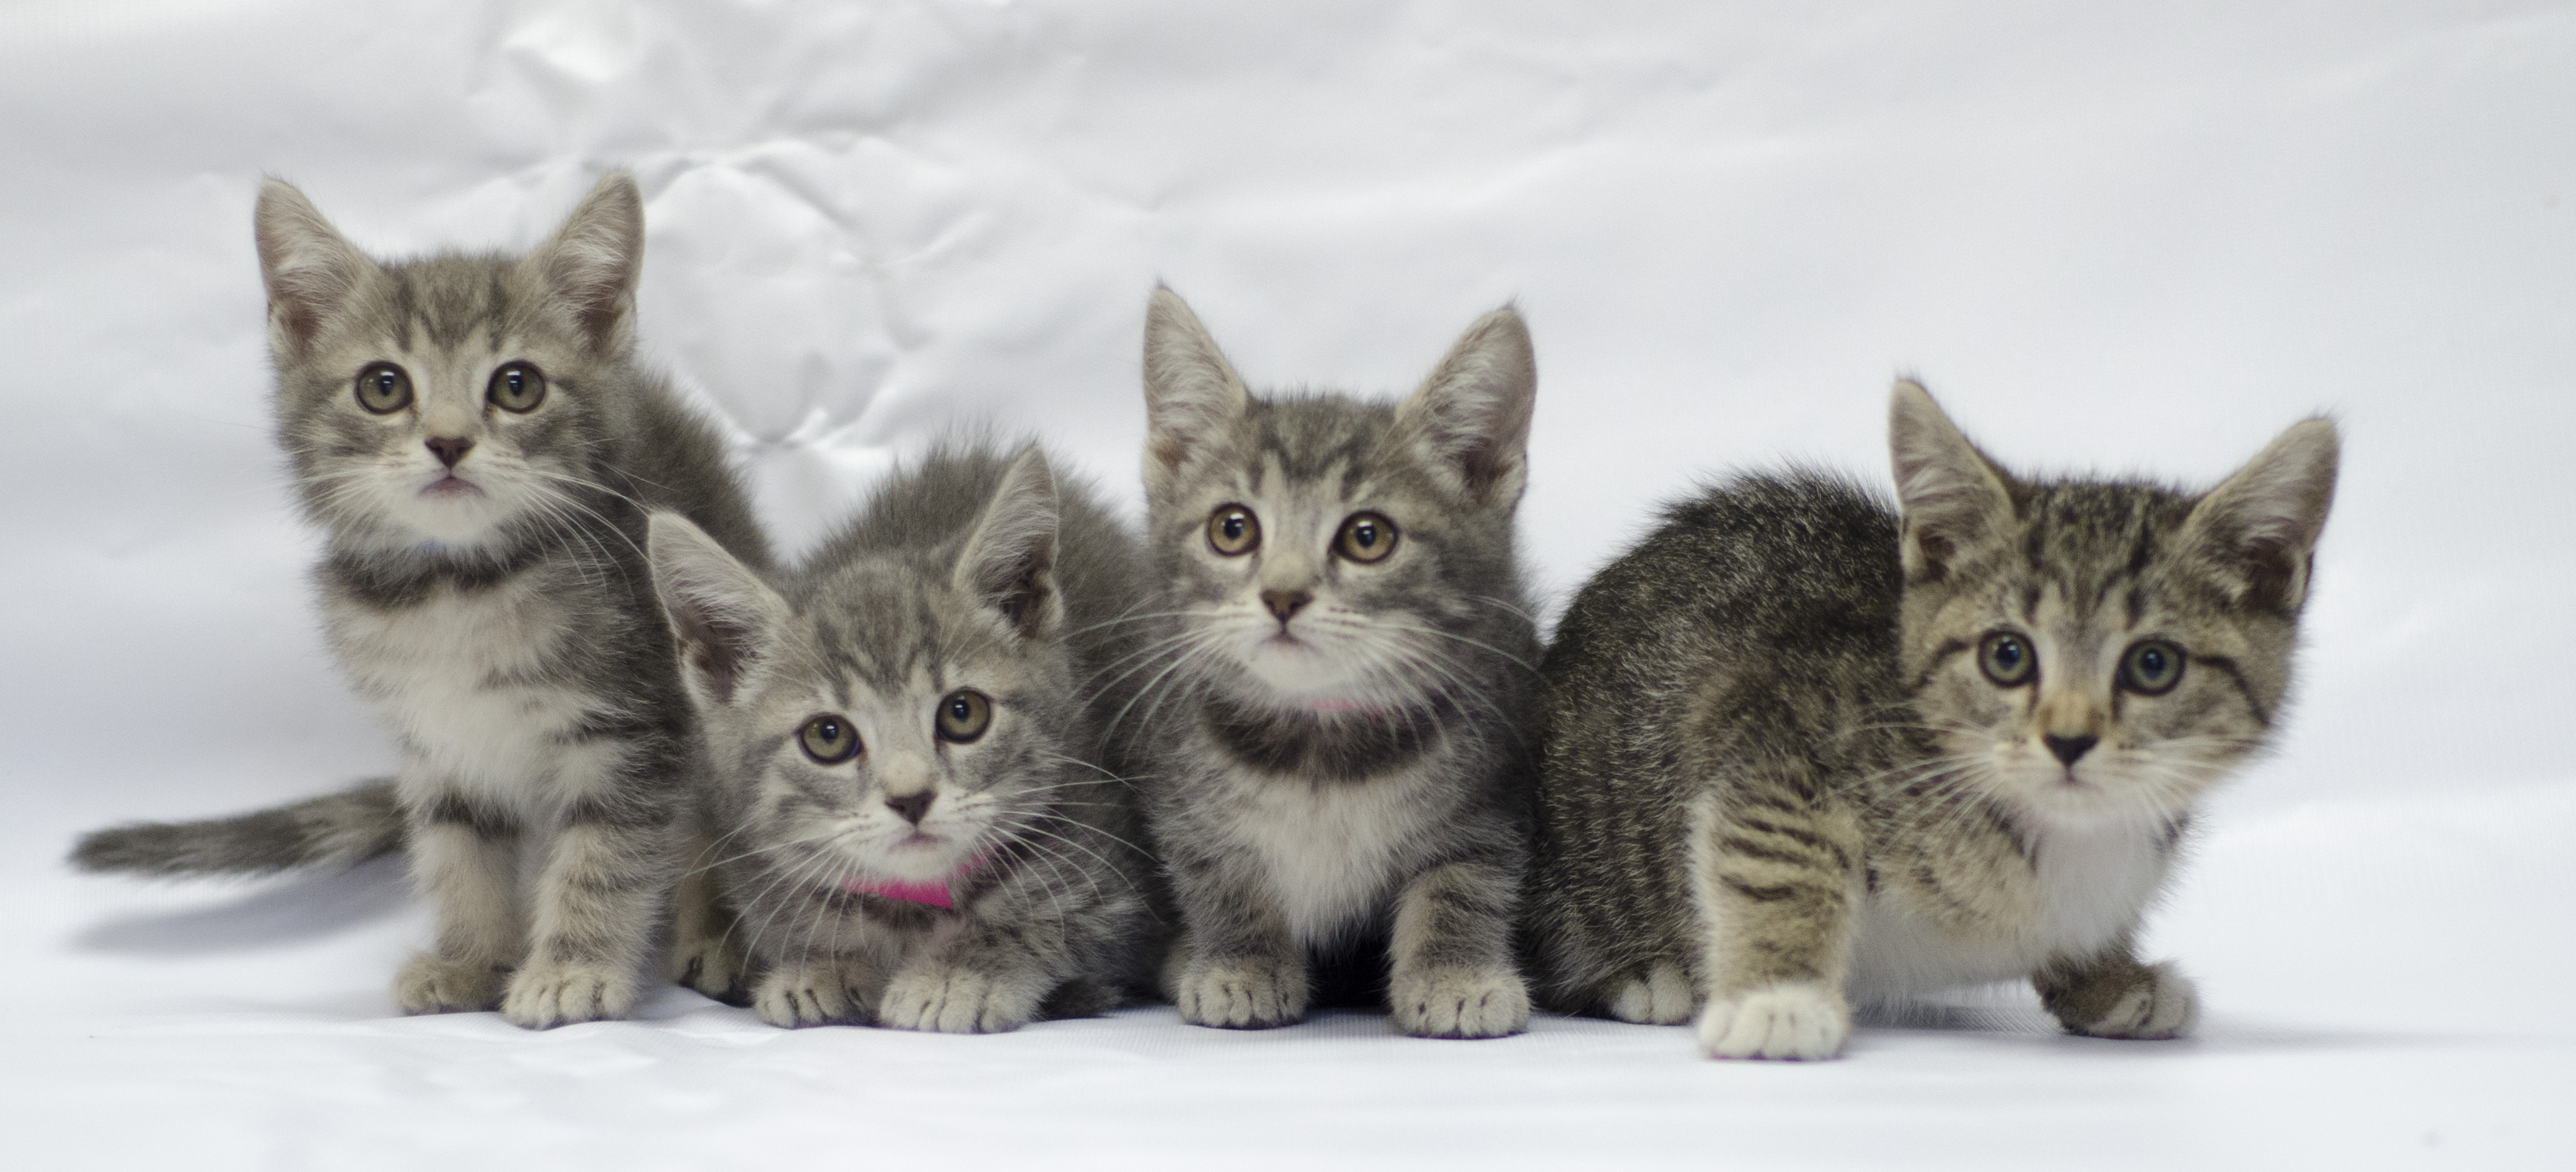
\includegraphics[width=1\linewidth]{4kittens.jpg}
  \end{figure}
  \end{block}
\end{frame}


\end{document}
